\section{Stromy}
Stromy jsou jedny z nejdůležitějších skupin grafů. Budeme je využívat v algoritmech stejně tak jako v mnoha datových strukturách. V této části si formálně zadefinujeme strom a podíváme se na jeho vlastnosti.

\begin{definition}
  Graf $G$ je \textbf{strom}, právě když je souvislý a acyklický.
\end{definition}

Strom je tedy libovolný souvislý graf, který neobsahuje kružnice.

Pro nesouvislý acyklický graf používáme název \textbf{les}.
\begin{definition}
  Graf $G$ je \textbf{les}, právě když je acyklický (nemusí být souvislý).
\end{definition}

\begin{definition}
  Vrchol $v$ v grafu $G$ nazveme \textbf{list}, pokud platí pokud $\deg_G(v) = 1$.
\end{definition}

List je tedy jakýkoli vrchol v libovolném grafu stupně 1. Ještě si dovolíme poznámku: V anglických textech se list (tedy \textit{leaf}) používá pouze pro vrcholy stupně 1 v lesích nebo stromech. V obecném grafu se nazývají \textit{pendent vertex}.


\vspace{1mm}
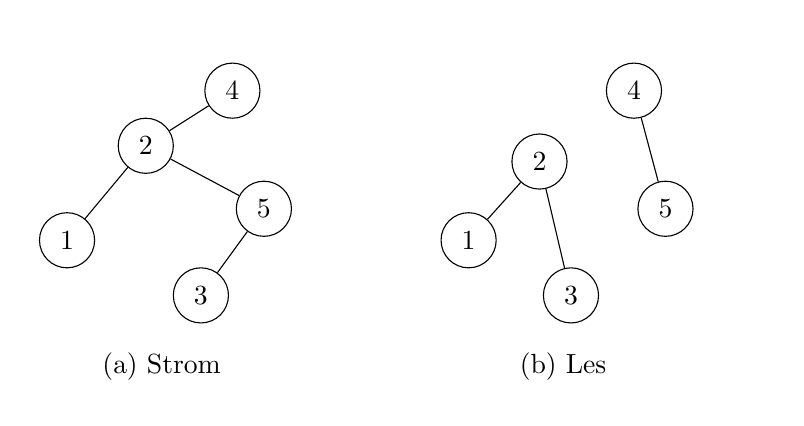
\begin{tikzpicture}[
    vnode/.style={circle, draw, minimum size=7mm, inner sep=0pt}
]
    % --- Graph (a) ---
    \node[vnode] (a2) at (0, 2) {2};
    \node[vnode] (a1) at (-1, 0.8) {1};
    \node[vnode] (a4) at (1.1, 2.7) {4};
    \node[vnode] (a5) at (1.5, 1.2) {5};
    \node[vnode] (a3) at (0.7, 0.1) {3};

    \draw (a2) -- (a1);
    \draw (a2) -- (a4);
    \draw (a2) -- (a5);
    \draw (a5) -- (a3);

    \node at (0.2, -0.8) {(a) Strom};

    % --- Graph (b) ---
    \node[vnode] (b2) at (5, 1.8) {2};
    \node[vnode] (b1) at (4.1, 0.8) {1};
    \node[vnode] (b3) at (5.4, 0.1) {3};
    \node[vnode] (b4) at (6.2, 2.7) {4};
    \node[vnode] (b5) at (6.6, 1.2) {5};

    \draw (b2) -- (b1);
    \draw (b2) -- (b3);
    \draw (b4) -- (b5);

    \node at (5.3, -0.8) {(b) Les};
    
    % Bounding box for padding
    \useasboundingbox (-1.5, -1.2) rectangle (8, 3.5);
\end{tikzpicture}
\vspace{0.5cm}

\subsection{Vlastnosti stromu}

\begin{theorem}[Věta o trhání listů]
Každý strom $T$ s alespoň $2$ vrcholy obsahuje alespoň dva listy.
\end{theorem}

\begin{proof}
Důkaz provedeme sporem.

\medskip
\noindent\textbf{Myšlenka důkazu:} Vybereme si nějakou nejdelší cestu ve stromě a tvrdíme, že její krajní vrcholy jsou listy. Pokud si představíte, jak taková cesta musí vypadat, mělo by být vidět, jak jsme k tomuto tvrzení dospěli. Spor získáme jednoduše tak, že tuto nejdelší cestu prodloužíme. Prodlužování nejdelších cest je velmi časté v důkazech sporem a jistě se vám bude ještě hodit.

\medskip
\noindent\textbf{Důkaz:} Pro spor nechť je graf $G$ strom a $P$ je nějaká nejdelší cesta v grafu $G$ s krajními vrcholy $u$ a $v$. Předpokládejme, že alespoň jeden z nich není list v grafu $G$.

BUNO $u$ je krajní vrchol, který není list. Musí tedy mít alespoň $2$ hrany (nemůže mít $0$, protože je součástí cesty). Označme $e = \{u,w\}$ hranu, která není obsažena v $P$. Nyní rozlišujeme dva případy:

\begin{enumerate}
    \item Pokud by $w$ byl součástí cesty $P$, pak by v grafu byl cyklus. To je spor s tím, že $G$ je strom (strom je acyklický).
    \item Pokud by $w$ součástí cesty nebyl, pak lze cestu $P$ prodloužit přidáním vrcholu $w$ za vrchol $u$. To je spor s předpokladem, že $P$ je nejdelší cesta v $G$.
\end{enumerate}

V obou případech jsme dospěli ke sporu. Tvrzení tedy platí.
\end{proof}